\subsection{Spectroscopic properties of silicon}

When an electron hole pair is recombining, the energy is released as a photon. By measuring this photon in a photo detector it can be determined how much energy that was released during recombination. This energy tells how large the band gap is, which in turn tells us something about the material. By shining light with high enough energy and intensity on to a sample, the light will excite electrons into all available states. When these states recombine, the emitted light can be detected by a camera as a spectra of different wavelengths. The fundamental energy gap between the valence and conduction bads in silicon is indirect, decreasing monotonically from 1.170~eV at 0~K to 1.125~eV at room temperature \cite{davies88}. The main phonon contribution (TO phonons) result in energies  around 1.1~eV for the emitted photons. If there are impurities or defects in the silicon crystal, they can in turn emit light at different photon energies. In order to generate electron-hole pairs, the sample can be excited by a laser. The laser wavelength have to be such that the energy of the light is larger than the band gap, in order to excite the sample. 



% band structure
% phonons
% Excitons
% EHD
% Different kinds of recombination in impurities/defects %% FIGURE (trap states, EHD, excitons etc.)
% Temperature dependance

% Spectroscopy (header)
% as method
% how to cool down a sample / cryo
% What is a cryostat
% different types of cooling, He, N etc.

% Excitation of sample
% different wavelengths, give list of inntrengingsdybde for forskjellige b�lgelengder
% spot size ++

\begin{figure}[H]
\centering
%\includegraphics[width=10cm,bb=0 0 306 265]{luminisence.png}%
\includegraphics[width=10cm]{luminisence}%
\caption{Excitation and recombination \cite{streetman}}%
\label{fig:luminescence}% 
\end{figure}

Figure \ref{fig:luminescence} show incoming light with high intensity in a direct band gap material. In $a$, an electron is excited to a high energy state, which falls down to a lower energy state in $b$, after a very short time. When this electron recombines in $c$, it emits a photon with energy equal to $E_c$. Another electron is excited in $d$, which reach a so-called trap state, which can occur from impurities in the crystal, or defects. This trap state have a lower energy than the band gap, and when this electron hole pair recombines, and lower energy is emitted. By looking at the light from such trap states, certain known spectra related to different impurities and defects can be recognized.

For an indirect band gap material like silicon, there are other important energy levels than the band gap to consider:

\subsubsection{Phonons}

A phonon is an elastic wave in a material such as a silicon crystal. It can be described as lattice vibrations, where the phonon propagate with wave vector $\vec{k}$. There is longitudinal (LA), transverse acoustical (TA), longitudinal (LO), and transverse optical (TO) modes. 

\begin{figure}[H]
\centering
\subfigure[Optical mode]{

\includegraphics[width=.45\columnwidth]{transvere_optical_mode}
\label{fig:transvere_optical_mode}
}
\subfigure[Acoustical mode]{
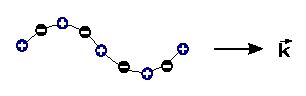
\includegraphics[width=.45\columnwidth]{transvere_acoustical_mode}
\label{fig:transvere_acoustical_mode}
}
\label{fig:transverse_phonon_modes}
\caption{Transverse phonon modes}
\end{figure}

The atoms in the crystal vibrate against each other, but their center of mass is fixed. If the two atoms carry opposite charges, we may excite a motion of transversal optical with the electric field of a light wave, so that the branch is called the optical mode (branch). If the atoms move together, as in long wavelength acoustical vibrations, whence the term acoustical mode (branch).

Since an electron-hole pair in silicon needs a phonon to recombine, the energy of which the emitted photon has, is highly dependant on the phonon energy involved, as well as the band gap. At absolute zero temperature, a crystal lattice lies in its ground state, and contains no phonons. A lattice at a non-zero temperature  has an energy that is not constant, but fluctuates randomly about some mean value. These energy fluctuations are caused by random lattice vibrations, which can be viewed as a gas of phonons. Due to a vast amount of phonons at room temperature, the energy released by recombination varies due to larger fluctuations. In silicon, the optical mode phonon energies are found right above 48 meV, transverse acoustic (TA) mode phonon energies are right below 25 meV, and LA modes are in between \cite{aksamija07}. \cite{davies88} list phonon energies in silicon as 

\begin{table}[H]
\centering
\begin{tabular}{cc}
18.4$\pm$0.2~meV & TA mode \\
56.2$\pm$1~meV & LO mode \\
58.0$\pm$1~meV & TO mode \\
\end{tabular}
\caption{Phonon modes in silicon from \cite{davies88}}
\label{tab:phonon_energies}
\end{table}


\subsubsection{Excitons}

An exciton is a quasi particle describing an electron bound to a hole. Electrons can be bound together by their attractive coulomb interaction, just as an electron is bound to a proton form a neutral hydrogen atom. An exciton can move through the crystal and transport energy, however it does not transport charge because it is electrically neutral.

\begin{figure}[H]
\centering
\includegraphics[width=\columnwidth]{exciton}%
\caption[Excitons]{The Mott-Wannier exciton usually free to move together through the crystal, and is weakly bound, with an average electron-hole distance large in comparison with the lattice constant. An ideal Frenkel exciton will travel as a wave throughout the crystal, but the electron is always close to the hole.}%
\label{fig:excitons}%
\end{figure}

Excitons can be formed in every insulating crystal. When the band gap is indirect, excitons near the direct gap may be unstable with respect to decay into a free electron and a free hole. All excitons are unstable with respect to the ultimate recombination process in which the electron drops and recombines with the hole. Excitons can also form complexes, such as a biexciton from two excitons \cite{kittel}. In the formation of excitons, the energy is lowered with respect to the binding energy of the exciton. For silicon, the binding energy of an exciton is 14.7~meV \cite{kittel}. In a tightly bound exciton (Frenkel) the excitation is localized on or near a single atom. The hole is usually on the same atom as the electron, although the pair may be anywhere in the crystal. Boron bound excitons have binding energy of 3.8~meV to the boron atom, and phosphorus bound excitons have binding energy 4.7~meV \cite{davies88} to the phosphorous atom.

\begin{figure}[H]
\centering
\includegraphics[width=\columnwidth]{exciton_levels}%
\caption[Excitation levels]{Exciton levels in relation to the conduction band edge for a simple band structure with both conduction and valence band edges at $\vec{k}$=0. Figure from \cite{kittel}}%
\label{fig:exciton_levels}%
\end{figure}

%% B bound, P bound, energy levels ?

\subsubsection{Electron-hole drops}

A condensed phase of an electron-hole plasma forms in Ge and Si when maintained at a low temperature and irradiated by light. When an electron-hole drop (EHD) forms, the absorption of a photon produces a free electron and free hole with high efficiency. These combine rapidly to form an exciton. If the exciton concentration is sufficiently high, most of the excitons will condense into a drop. The binding energy relative to free exciton is 9.3~meV in silicon with 3.5\cdot10$^{18}$~cm$^{-3}$ $n$ or $p$ at 23K \cite{kittel}.


%% figure with multiple bandgap shortages present



\subsubsection{Pumping wavelength}

Pumping light needs to have enough energy to fill all available states in the crystal lattice, in order to detect defects and impurities. For silicon, which has an ideally forbidden band gap of around 1.22~eV at 0~K \cite{streetman}, has impurity/defect bands below this band gap. In order to fill these states, the pumping wavelength should be below 1017~nm, which corresponds to energies just over 1.22~eV.

Silicon has different absorption lengths for different wavelengths. Absorption length is about 1~$�$m for 532~nm laser excitation, which means that precipitates, and defects deeper in the sample like iron precipitates won't be detected \cite{gundel09}. By comparison, 800~nm, reach 12~$�$m into the sample, and 1125~nm reach as far down as 200~$�$m \cite{laserdybde}.


\subsubsection{Spot size}

Having a small diameter on the pumping laser allows for a high resolution of characteristics on the sample. In an iron contaminated sample, \cite{gundel09} show that at some distinct spots of a size between 1$�$m and 4$�$m, the band to band photoluminescence peak is particular low at spots with iron precipitates. 

A large electron hole droplet could overshadow characteristics from impurities in the sample. \cite{satoshi04} show that electron hole droplets become more intense for a smaller volume, with a silicon nanolayer smaller than the absorption depth of the laser. \cite{satoshi04} used a 488~nm pumping laser with 1,5~$�$m diameter, on silicon nanolayer thickness of 50~nm and 340~nm. For the 50~nm layer, \cite{satoshi04} observed a large electron hole droplet, even for small pumping intensities, with the same amount of photo excited carriers per volume as for the 340~nm layer. Assuming that a small volume give rise to a larger electron hole droplet, it would be a limiting factor for the spot size and pumping wavelength.

\subsubsection{Laser intensity}

High excitation laser intensity gives a high signal to noise ratio. But with a large pumping intensity, an electron hole droplet become visible in the specter around 1.08~eV in bulk silicon \cite{hammond75}. This electron-hole drop is also more intense at small volumes. \cite{satoshi04} show that electron hole droplets occur at weak excitations (0.75~mW) and even at high temperatures for a silicon nanolayer of 50nm. For thickness of 340~nm, the electron hole droplet show up at pumping intensity of 3~mW and above, and the intensity of the electron hole droplet grow larger than for the free exciton at 15~mW. This electron hole droplet is not wanted, as it can mask characteristic photoluminescence from impurities.

With a larger pumping intensity, the impurity photoluminescence would in some cases also increase. Photoluminescence from chromium bound with a boron atom is known to increase linearly with laser power \cite{conzelmann82,conzelmann83}, and would be easier to detect at a higher pumping intensity.

Temperature increase is also an issue with high laser intensity. When hitting a small area on the sample, the temperature in that particular area will rise rapidly unless subject to heavy cooling. This can lead to material stress, and broadening of the luminescence energy spectra due to different phonon energies.


\subsubsection{Temperature dependency}

At room temperature, there's a large probability that the phonon energy involved in recombination has an energy considerably different from the mean value, compared to temperatures close to 0K. This makes it difficult to separate phonon assisted recombination, from other available states, like direct recombination from trap states. Trap states are important because they describe impurities by exact photon energies, which in turn makes it possible to recognize known impurities. But any recombination involving phonons will have a substantial broadening in regards to energy at room temperature.

To overcome the problem of distributed phonon energies, the sample can be cooled down. When cooling down, there are less phonon states available, leading to a much narrower energy distribution of the phonons. This is desirable when looking at the photoluminescence, in order to recognize known spectra. Due to the low binding energies involved in silicon, individual lines would be next to impossible to detect without very low temperatures.

Low temperatures, and high exciting laser light intensity can lead to electron-hole drops. Temperature is a substantial limiting factor for measuring silicon luminescence spectra, meaning low temperature is key to analyze silicon photoluminescence. Electron-hole drops are undesirable because they don't carry information about the material itself, and can emit light at the same wavelengths as actual material properties would. This is a limiting factor at low temperatures on the laser intensity, spot size, and wavelength.

A common way to cool down a sample, is to use liquid nitrogen. Nitrogen has a boiling temperature of 77K, so by exposing the sample to boiling nitrogen, it is cooled down. This can be done is a cryostat, which essentially is a vacuum chamber with a sample holder, where the sample holder is being cooled down. This way there will be no nitrogen contaminants on the sample itself, with only the sample holder being cooled down by nitrogen directly. It's also common to mount the sample holder on piezo elements, which can be used to move the sample in xyz directions. 

For silicon, 77K still leads to substantial broadening of emitted photon energies. In order to reach lower temperatures, a different coolant can be used. By using helium, which has a boiling temperature of 4.2K, the energy broadening is reduced to negligible values, and sharp lines from the photoluminescence can be detected.
%% To solve this -- low temperatures -- cryostat -- Helium, Nitrogen, bathind in liquid helium, compared to cryostat - cryo cryo lala